\section{Work packages}
\label{sec:workpackages}

This section is future work \evfut{} throughout. WP1--WP11 derive from the phased roadmap in
\cref{sec:roadmap} and from the validation program's studies V0--V8 (\cref{sec:validation}).
Months count from the start of Phase~1 (M1). Phase~0 comes before M1 and before any grant; it is
owner-run and marked P0. Phase~1 runs M1--M14 and ends at MS3. Phase~2 runs M15--M48 and starts
only if MS3 reads continue; if Phase~2 is a separate award, its months shift by the funder's
review time.

\Cref{fig:gantt} gives the schedule and dependencies as one diagram. \Cref{tab:milestones} gives
the gates. Each work package below gives its phase, objective, key tasks, deliverables, milestones
and main risks. Person-months per phase are in \cref{sec:resources}; roles are in \cref{sec:team}.

\begin{figure}[tbp]
  \centering
  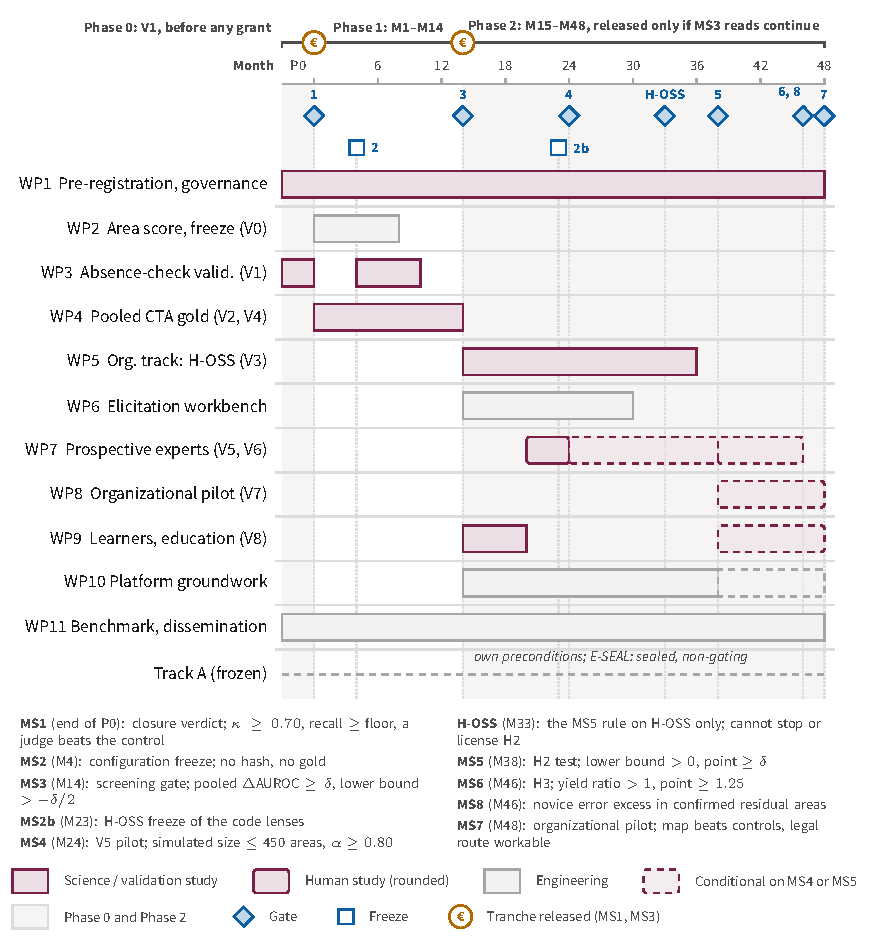
\includegraphics{figures/pdf/fig15_gantt.pdf}
  \caption[Work package schedule]{Work packages by phase, with gates as diamonds, the MS2 and MS2b
  freezes as squares, and the tranche releases at MS1 and MS3 as coins. Phase~0 (before
  M1, owner-run) ends at MS1, the closure verdict. Phase~1 (M1--M14) builds the area score,
  freezes the configuration at MS2 (about M4), and only then acquires gold; it ends at MS3
  (about M14). Phase~2 bars (M15--M48) are
  released only if MS3 reads continue. Inside Phase~2, V5's main study waits for MS4, and V6, V7
  and V8c wait for MS5. The organizational track freezes its code lenses at MS2b and reads H-OSS
  at its own gate. Validation Track A runs on its own preconditions and is not scheduled by this
  chart.}
  \label{fig:gantt}
\end{figure}

\footnotesize

\paragraph{WP1 -- Pre-registration, governance and data protection (P0, Phases 1--2)}
\mbox{}\par
\begin{tabularx}{\linewidth}{@{}>{\bfseries}p{2.6cm}X@{}}
  \toprule
  Objective & Every gate is fixed before its data exist, an independent reader checks it, and
    every human-data step is legal. \\
  Key tasks & P0: hash-commit the V1 pre-registration (codebook, $\kappa$ floor, retrieval-recall
    floor, judge margin, analysis script) before coding; appoint the external gate reader before
    MS1 is read. Phase~1: fill the threshold table ($\delta = 0.05$ recommended,
    \cref{sec:validation}); pre-register V0, V2 and V4, including V2's pooled and incremental
    analysis and the list of eligible golds; license checks; the budget headroom rule
    (\cref{sec:resources}); per-domain eligibility registers. Phase~2: ethics for V5, V6 and V8c,
    submitted at M15; V5 pre-registered at the powered size (M24); H-OSS (M23) and V6 (M38)
    pre-registrations; DPIA and works-council preparation for V7 after MS5. \\
  Deliverables & V1 pre-registration (P0); threshold table and V0/V2/V4 pre-registrations (M4);
    ethics approval for V5/V6 (M19); V5 pre-registration (M24); DPIA and data agreement for V7
    (M42); final data-management and open-data report (M48). \\
  Milestones & MS2 (M4, shared with WP2). \\
  Main risks & Thresholds set after data are seen; ethics delay pushes V5; legal cost of V7. \\
  \bottomrule
\end{tabularx}

\paragraph{WP2 -- Area score, configuration freeze and deferred N2 validation (V0; Phase~1)}
\mbox{}\par
\begin{tabularx}{\linewidth}{@{}>{\bfseries}p{2.6cm}X@{}}
  \toprule
  Objective & Make pipeline outputs admissible as inputs to a gold test (L0), and give the gap map
    an area-level score, which the PoC does not produce. \\
  Key tasks & Build a pre-registered area score from the \emph{uncapped} candidate set within an
    area (for example max or noisy-OR over candidate scores), chosen on PLC and GDPR pilot data
    only. Check that it is not a monotone function of area size or source density, and report its
    partial correlation with density. Add an \code{--areas} input at task-step grain. Build
    admissibility checks as code. Build dated-corpus mode (its source and date rule are in
    \cref{sec:validation}) with a gold blocklist, and count the dated sources each candidate gold
    reaches. Run the deferred N2 protocols as registered (E-LIVE v3, E-PLANT run 2, E-ABST run
    2). Then freeze: the judge chosen at MS1, lexicons, thresholds, the area score and the list of
    eligible golds are hash-committed together at MS2. Depends on MS1 and WP1. \\
  Deliverables & Area score, admissibility checker and dated-corpus source pilot (M3); frozen
    configuration hash (M4); N2 deferred-validation report (M8). \\
  Milestones & MS2 (M4): no hash, no gold. \\
  Main risks & Live runs expose new defects, as they did in N2; dated corpora too small for a
    gold domain; the area score tracks density. \\
  \bottomrule
\end{tabularx}

\paragraph{WP3 -- Absence-check validation (V1 in P0; judge text-type check in Phase~1)}
\mbox{}\par
\begin{tabularx}{\linewidth}{@{}>{\bfseries}p{2.6cm}X@{}}
  \toprule
  Objective & Decide whether \enquote{is this element really unsaid?} can be judged reliably,
    by humans and by a judge, and whether retrieval finds the element where it is stated (L1). \\
  Key tasks & P0 (owner-run): write a closure codebook with anchors per lens. Code the 107
    admissible lens firings in both arms of the fair control, plus about 100 units from one new
    non-gold domain; the owner (under origin blinding) and one non-owner coder code every unit.
    Report weighted human--human $\kappa$ on three states, gated on closed versus not closed. For
    about 50 firings, search the ledger's full snapshots for the missing element and report
    retrieval recall. Score a judge panel (the local 7B model, a stronger open-weight judge, and
    frontier judges from other families) against the fair control. Phase~1: before any gold is
    unsealed, double-code a closure sample from each dated V2 reconstruction, to check the MS1
    judge on that text type; where it fails, closure there is human-coded. \\
  Deliverables & Codebook and V1 pre-registration (P0); closure set, released, and closure verdict
    report (end of P0); judge text-type report (M10). \\
  Milestones & MS1 (end of P0): the closure verdict. \\
  Main risks & Human--human $\kappa$ below 0.70 (the construct itself is unreliable); low
    retrieval recall; the judge overfits the codebook; the judge fails on the new text type. \\
  \bottomrule
\end{tabularx}

\paragraph{WP4 -- Pooled retrospective CTA gold test and residual check (V2, V4; Phase~1)}
\mbox{}\par
\begin{tabularx}{\linewidth}{@{}>{\bfseries}p{2.6cm}X@{}}
  \toprule
  Objective & Screen H2 on several published CTA golds before any expert is recruited (L2), and
    test whether the residual can be measured at all (L3). \\
  Key tasks & Check itemized gold availability by metadata and author contact only; the list of
    eligible golds (at least three proposed) is fixed at MS2. Build area partitions from dated
    pre-gold sources. After MS2, reconstruct on each dated corpus, then acquire each gold,
    sealed. Run per-item memorization
    probes and exclude probe-positive items. Map gold items to areas by blind double coding. Pool
    $\Delta$AUROC across golds by random effects, against the strongest baseline chosen inside
    each bootstrap resample. Test the map's incremental value over density and area size. Run the
    V4 known-truth check on V2 data. \\
  Deliverables & Gold availability report (M3); dated-corpus reconstructions (M10); pooled V2
    result and V4 report (M13); a public reconstruct-vs-CTA benchmark release (M16). \\
  Milestones & MS3 (M14). \\
  Main risks & Fewer than three eligible golds; contamination; unmappable gold items; wide pooled
    intervals. \\
  \bottomrule
\end{tabularx}

\begin{keyquestionbox}
  \textbf{MS3, about M14 -- the screening gate for Phase~2 money.} The external gate reader reads
  the pooled V2 result against the pre-registration. Phase~2 is released only if the point
  estimate is at least $\delta$, the lower 90\% bound is above $-\delta/2$, and the map adds value
  over density and area size. Otherwise H2 funding stops, no Phase~2 work package starts, and the
  interview-only pivot is proposed on its own budget. MS3 does not decide H2; MS5 does.
\end{keyquestionbox}

\paragraph{WP5 -- Organizational track: developer-departure study (V3, H-OSS; Phase~2)}
\mbox{}\par
\begin{tabularx}{\linewidth}{@{}>{\bfseries}p{2.6cm}X@{}}
  \toprule
  Objective & Test H-OSS: the gap map, adapted to code and commit evidence, predicts where
    knowledge is lost when developers leave. H-OSS is a separate hypothesis; it cannot kill or
    license H2. \\
  Key tasks & Build a World B Git adapter (commits, blame at time $t$, issues, pull requests,
    reviews, dated documentation) for public repositories. Develop code lenses on repositories
    outside the departure sample, and freeze them at MS2b (M23), after the adapter exists. Validate the
    closure judge on commit and issue text, or register V3 without closure. Pilot five departures
    to estimate the base rate, clustering and coding time; decide power. Run the main study if
    feasible, else register it as descriptive. Blind double code rationale-seeking issues and
    defect-fix commits; use a staggered-adoption difference-in-differences estimator
    \evlit{} \parencite{callaway2021difference}. Depends on WP1 (pseudonymization record). \\
  Deliverables & Git adapter with provenance (M22); code-lens freeze (M23); pilot and power
    decision (M26); H-OSS result (M33); coded post-departure dataset, pseudonymized (M36). \\
  Milestones & MS2b (M23); the H-OSS gate (M33), which uses the MS5 rule on H-OSS only. \\
  Main risks & Too few departures with enough later activity; authorship metrics may break under
    agentic coding; target repositories sit in model pretraining data. \\
  \bottomrule
\end{tabularx}

\paragraph{WP6 -- Elicitation workbench (research prototype; Phase~2)}
\mbox{}\par
\begin{tabularx}{\linewidth}{@{}>{\bfseries}p{2.6cm}X@{}}
  \toprule
  Objective & Build the minimum software that V5 and V6 need to run blind, logged, and codable. \\
  Key tasks & A question service (template questions now; expected-information-gain selection
    later, future work N6) with a fixed unknown-unknowns fraction; blind-arm separation, so the
    interviewer view never shows scores or strata; World C records into the ledger; a segmentation
    and coding tool with blinding checks; residual accounting and cost per validated item. The
    Track A turn contract, leading-question guard and corroboration code are copied into the new
    package; \code{instrument/} is never imported. Starts at M15, after MS3. \\
  Deliverables & Workbench v1, tested on simulated labeled sessions (M21); v2 for two domains
    (M30). \\
  Milestones & MS4 (M24) is the first gate to use it. \\
  Main risks & Leakage of scores or strata into the interviewer or coder views. \\
  \bottomrule
\end{tabularx}

\paragraph{WP7 -- Prospective expert validation (V5, V6; Phase~2)}
\mbox{}\par
\begin{tabularx}{\linewidth}{@{}>{\bfseries}p{2.6cm}X@{}}
  \toprule
  Objective & Decide H2 on fresh, blind human elicitation (L4), and test H3, whether targeting
    saves expert time (L5a). \\
  Key tasks & V5 pilot: 6 experts
    $\times$ 20 areas in PLC (40 areas, three experts each), not analyzed for effect; it measures
    prevalence, design effect, coding time and leakage (M21--M24). V5 main (M25--M37), sized for
    $\delta = 0.05$: about 300 areas (about 150 per class) in two held-out subdomains (D3, D4),
    strata G/D/L/R, and short neutral CDM probes of about 8 minutes
    \evlit{} \parencite{klein1989critical}. Each area is probed by 3 experts
    \evlit{} \parencite{chao1994percentage}, and each expert covers about 20 areas, so about 45
    experts are needed. V6 (M39--M45), only after MS5 reads continue: a
    targeted-versus-untargeted crossover with question-seeded coding against leading questions
    \evlit{} \parencite{loftus1975leading}. \\
  Deliverables & V5 pilot report and powered sample (M24); V5 main result
    (M38); V6 result (M46); residual corpus v1 (M46). \\
  Milestones & MS4 (M24); MS5 (M38), the H2 verdict; MS6 (M46), the H3 verdict. \\
  Main risks & Recruiting about 45 experts; a prevalence below one half, which raises the areas
    needed above MS4's funded ceiling; coding time; interviewer effects. \\
  \bottomrule
\end{tabularx}

\paragraph{WP8 -- Organizational pilot (V7; Phase~2)}
\mbox{}\par
\begin{tabularx}{\linewidth}{@{}>{\bfseries}p{2.6cm}X@{}}
  \toprule
  Objective & Test transfer to one partner organization (L5b) and whether the legal route is
    workable. \\
  Key tasks & Select a partner (a software organization first); complete a DPIA and a
    legitimate-interest balancing test; secure a works agreement where German co-determination
    applies; agree a data contract (no training on partner data; on-prem or equivalent hosting).
    Run the retrospective part (past departures or onboarding tickets as the outcome; the H-OSS
    design, if H-OSS has run) and the prospective part (the V5 design, on one or two critical
    units). Starts only after MS5 reads continue and the deferred N2 validation is complete.
    Depends on WP10's on-prem stack and WP1's legal groundwork. \\
  Deliverables & Signed partner and data agreements (M42); retrospective result (M45);
    prospective result and feasibility report (M48). \\
  Milestones & MS7 (M48). \\
  Main risks & Partner access; a works-council veto; staff reading the tool as surveillance;
    prompt injection through internal documents \evlit{} \parencite{greshake2023not}. \\
  \bottomrule
\end{tabularx}

\paragraph{WP9 -- Learner link and education pilot (N4, V8a, V8c, E-SEAL; Phase~2)}
\mbox{}\par
\begin{tabularx}{\linewidth}{@{}>{\bfseries}p{2.6cm}X@{}}
  \toprule
  Objective & Test whether the expert residual relates to learner difficulty, and whether
    teaching validated residual items changes anything measurable. \\
  Key tasks & (a) V8a on public mathematics data, after license checks (M15--M20). (b) An E-SEAL
    interface to Track A: sealed gap-map scores, added only if the Track A owner approves before
    Stage A. (c) V8c: 30--60 novices in a validated V5 domain, after a 10-novice pilot; it starts
    only after MS5 reads continue (M39--M45). (d) An education materials pilot built only from
    validated items, run as a manipulation check on one course section or apprentice cohort, not
    as a powered RCT (M45--M48). \\
  Deliverables & V8a report (M20); V8c result (M46); education pilot feasibility report and an
    RCT pre-registration draft (M48). \\
  Milestones & MS8 (M46). \\
  Main risks & Non-commercial data licenses; a null learner link, which is plausible and
    informative; learner data protection. \\
  \bottomrule
\end{tabularx}

\paragraph{WP10 -- Platform groundwork and World B infrastructure (Phase~2)}
\mbox{}\par
\begin{tabularx}{\linewidth}{@{}>{\bfseries}p{2.6cm}X@{}}
  \toprule
  Objective & Turn the PoC's properties into the platform's core, without building features ahead
    of evidence. \\
  Key tasks & A typed run-status record, replacing the untyped sidecar; ledger storage that scales
    beyond one JSON file per run, which V5's volume needs. After MS5 reads continue: an on-prem
    stack spanning three model families (generator, verifier, closure judge); access-control
    propagation to labels (a claim inherits its evidence's most restrictive access control); an
    erasure design (pseudonym key kept outside the ledger); a hash-chained audit trail. \\
  Deliverables & Typed run status and scalable ledger (M24); on-prem judge stack (M43); access
    control, erasure and audit for the WP8 tenant (M46); a platform decision record for S6,
    written only if MS5 and MS7 read continue (M48). \\
  Milestones & Supports MS7. \\
  Main risks & Building for customers before MS5 reads; on-prem judges weaker than hosted ones. \\
  \bottomrule
\end{tabularx}

\paragraph{WP11 -- Open benchmark, residual corpus and dissemination (all phases)}
\mbox{}\par
\begin{tabularx}{\linewidth}{@{}>{\bfseries}p{2.6cm}X@{}}
  \toprule
  Objective & Make the program's outputs reusable whatever the gates read. \\
  Key tasks & Release the closure set, the reconstruct-vs-CTA benchmark, the coded post-departure
    dataset, a consented subset of the residual corpus, and every pre-registration and negative
    result. Publish a paper after each gate. Licenses and consent are cleared by WP1. \\
  Deliverables & Releases at the end of P0 (closure set), M16, M36, M46 and M48; papers after MS1,
    MS3, MS5, MS6, MS7 and the H-OSS gate. \\
  Milestones & Tied to the releases above. \\
  Main risks & Gold licenses that forbid redistribution; mitigated by releasing mappings and code,
    never the gold text itself. \\
  \bottomrule
\end{tabularx}

\normalsize

\FloatBarrier
\subsection{Milestones}

\Cref{tab:milestones} lists every gate in time order, with its phase, its month and the rule that
reads it. The external gate reader reads MS1, MS3 and MS5, and signs off any owner exception
at any gate (\cref{sec:team}).

\begin{table}[!htbp]
  \centering
  \small
  \caption{Milestones in time order: phase, month, and the rule that reads each gate. MS1
  releases Phase~1, MS3 releases Phase~2, and MS5 decides H2. MS2 and MS2b are freezes: no hash,
  no data.}
  \label{tab:milestones}
  \begin{tabularx}{\linewidth}{@{}lllX@{}}
    \toprule
    Milestone & Phase & Month & Gate rule \\
    \midrule
    MS1 & 0 & P0 end & \textbf{Closure verdict.} Continue if human $\kappa\geq0.70$, recall meets
      its floor, and one judge beats the fair control by the margin; this releases the Phase~1
      proposal. Otherwise stop the automated absence check and take a pivot. \\
    MS2 & 1 & M4 & Configuration freeze: MS1's judge, lexicons, thresholds, area score, the V0,
      V2 and V4 pre-registrations and the list of eligible golds hash-committed. No gold before
      it. \\
    MS3 & 1 & M14 & \textbf{Screening gate.} Release Phase~2 only if the pooled $\Delta$AUROC point
      estimate is $\geq\delta$, its lower 90\% bound is $>-\delta/2$, and the map adds value over
      density and area size. Otherwise stop H2 funding. \\
    MS2b & 2 & M23 & H-OSS freeze: code lenses and the H-OSS pre-registration hash-committed, after
      the Git adapter exists. \\
    MS4 & 2 & M24 & V5 pilot: the projected number of areas fits the funded ceiling of 450,
      segmentation $\alpha\geq0.80$, and stratum guessing stays near chance. \\
    H-OSS & 2 & M33 & The MS5 rule, applied to H-OSS only; it can neither stop nor license H2. \\
    MS5 & 2 & M38 & \textbf{H2 verdict.} Stop if the upper 90\% bound $<\delta$; continue if the
      lower bound $>0$ and the point estimate $\geq\delta$; otherwise not supporting H2, and H2
      funding ends. \\
    MS6 & 2 & M46 & H3: yield-ratio lower bound $>1$ and point estimate $\geq1.25$ (the smallest
      effect size of interest, SESOI); any other reading counts against H3. \\
    MS8 & 2 & M46 & Novice error excess in confirmed residual areas. \\
    MS7 & 2 & M48 & Organizational pilot: the map beats density and random controls in both parts;
      the legal route is workable. \\
    \bottomrule
  \end{tabularx}
\end{table}
\FloatBarrier
